\documentclass{article}
\usepackage{graphicx}

\begin{document}

\title{The White Whale}
\author{Herman Melville}
\maketitle

\section*{The Captain}

 But as the strange captain, leaning over the pallid bulwarks, was in the act of putting his trumpet to his mouth, it somehow fell from his hand into the sea; and the wind now rising amain, he in vain strove to make himself heard without it. Meantime his ship was still increasing the distance between. While in various silent ways the seamen of the Pequod were evincing their observance of this ominous incident at the first mere mention of the White Whale's name to another ship, Ahab for a moment paused; it almost seemed as though he would have lowered a boat to board the stranger, had not the threatening wind forbade. But taking advantage of his windward position, he again seized his trumpet, and knowing by her aspect that the stranger vessel was a Nantucketer and shortly bound home, he loudly hailed -- 'Ahoy there! This is the Pequod, bound round the world! Tell them to address all future letters to the Pacific ocean! and this time three years, if I am not at home, tell them to address them to -- -- '

\section{More on the Ocean}

   At that moment the two wakes were fairly crossed, and instantly, then, in accordance with their singular ways, shoals of small harmless fish, that for some days before had been placidly swimming by our side, darted away with what seemed shuddering fins, and ranged themselves fore and aft with the stranger's flanks. Though in the course of his continual voyagings Ahab must often before have noticed a similar sight, yet, to any monomaniac man, the veriest trifles capriciously carry meanings. 

\begin{figure}[!htp]
  \begin{center}
    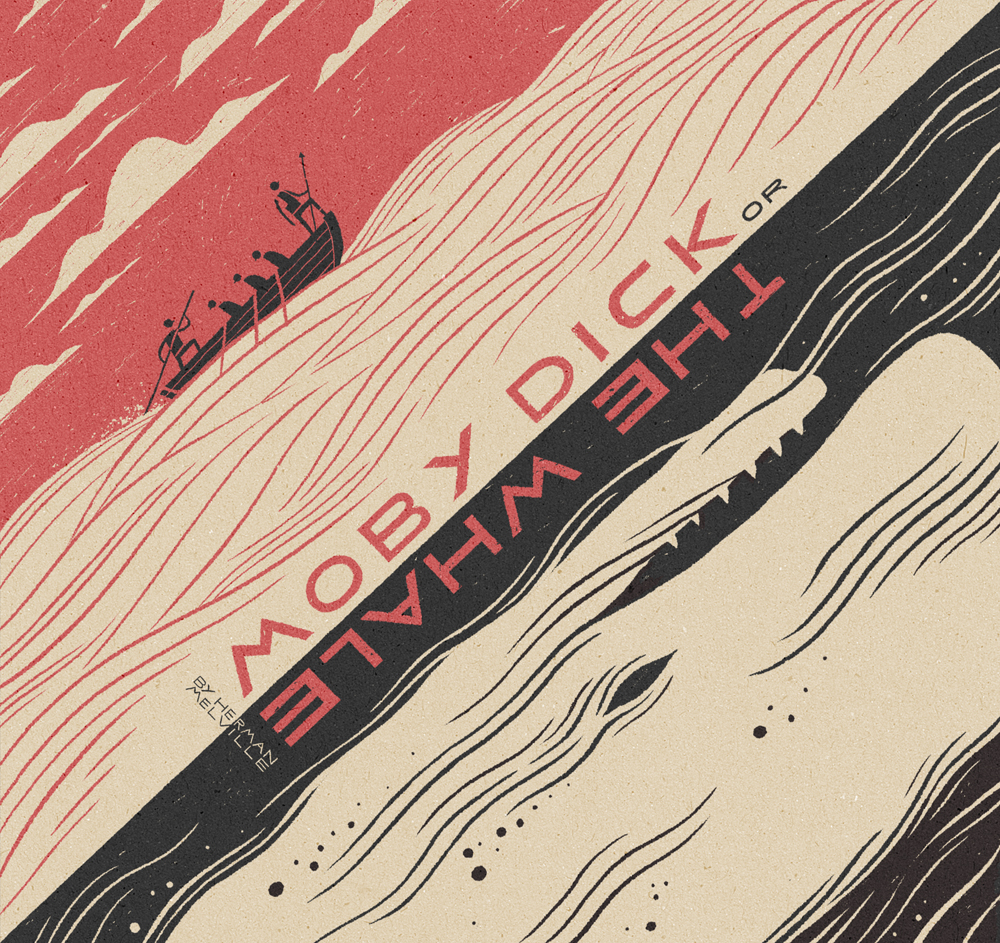
\includegraphics{moby-dick-done}
    \caption{
        \textbf{Moby Dick, or, the Whale.}
My soul is more than matched; she's overmanned; and by a madman! Insufferable sting, that sanity should ground arms on such a field! But he drilled deep down, and blasted all my reason out of me! I think I see his impious end; but feel that I must help him to it. Will I, nill I, the ineffable thing has tied me to him; tows me with a cable I have no knife to cut. Horrible old man! Who's over him, he cries;—aye, he would be a democrat to all above; look, how he lords it over all below! Oh! I plainly see my miserable office,—to obey, rebelling; and worse yet, to hate with touch of pity! For in his eyes I read some lurid woe would shrivel me up, had I it. Yet is there hope. Time and tide flow wide. The hated whale has the round watery world to swim in, as the small gold-fish has its glassy globe. His heaven-insulting purpose, God may wedge aside. I would up heart, were it not like lead. But my whole clock's run down; my heart the all-controlling weight, I have no key to lift again. 
    }
  \end{center}
\end{figure}

Now, how had this noble rescue been accomplished? Why, diving after the slowly descending head, Queequeg with his keen sword had made side lunges near its bottom, so as to scuttle a large hole there; then dropping his sword, had thrust his long arm far inwards and upwards, and so hauled out our poor Tash by the head. He averred, that upon first thrusting in for him, a leg was presented; but well knowing that that was not as it ought to be, and might occasion great trouble; -- he had thrust back the leg, and by a dexterous heave and toss, had wrought a somerset upon the Indian; so that with the next trial, he came forth in the good old way -- head foremost. As for the great head itself, that was doing as well as could be expected.

   And thus, through the courage and great skill in obstetrics of Queequeg, the deliverance, or rather, delivery of Tashtego, was successfully accomplished, in the teeth, too, of the most untoward and apparently hopeless impediments; which is a lesson by no means to be forgotten. Midwifery should be taught in the same course with fencing and boxing, riding and rowing.

   I know that this queer adventure of the Gay-Header's will be sure to seem incredible to some landsmen, though they themselves may have either seen or heard of some one's falling into a cistern ashore; an accident which not seldom happens, and with much less reason too than the Indian's, considering the exceeding slipperiness of the curb of the Sperm Whale's well.

\begin{figure}[!htp]
  \begin{center}
      \includegraphics{whale-8546-svg}
    \caption{
        \textbf{Sperm whale}
        A sperm whale, in svg.
    }
  \end{center}
\end{figure}

   But, peradventure, it may be sagaciously urged, how is this? We thought the tissued, infiltrated head of the Sperm Whale, was the lightest and most corky part about him; and yet thou makest it sink in an element of a far greater specific gravity than itself. We have thee there. Not at all, but I have ye; for at the time poor Tash fell in, the case had been nearly emptied of its lighter contents, leaving little but the dense tendinous wall of the well -- a double welded, hammered substance, as I have before said, much heavier than the sea water, and a lump of which sinks in it like lead almost. But the tendency to rapid sinking in this substance was in the present instance materially counteracted by the other parts of the head remaining undetached from it, so that it sank very slowly and deliberately indeed, affording Queequeg a fair chance for performing his agile 
   obstetrics on the run, as you may say. Yes, it was a running delivery, so it was.

      Now, had Tashtego perished in that head, it had been a very precious perishing; smothered in the very whitest and daintiest of fragrant spermaceti; coffined, hearsed, and tombed in the secret inner chamber and sanctum sanctorum of the whale. Only one sweeter end can readily be recalled -- the delicious death of an Ohio honey-hunter, who seeking honey in the crotch of a hollow tree, found such exceeding store of it, that leaning too far over, it sucked him in, so that he died embalmed. How many, think ye, have likewise fallen into Plato's honey head, and sweetly perished there? 


 When gliding by the Bashee isles we emerged at last upon the great South Sea; were it not for other things, I could have greeted my dear Pacific with uncounted thanks, for now the long supplication of my youth was answered; that serene ocean rolled eastwards from me a thousand leagues of blue.

\begin{figure}[!htp]
  \begin{center}
      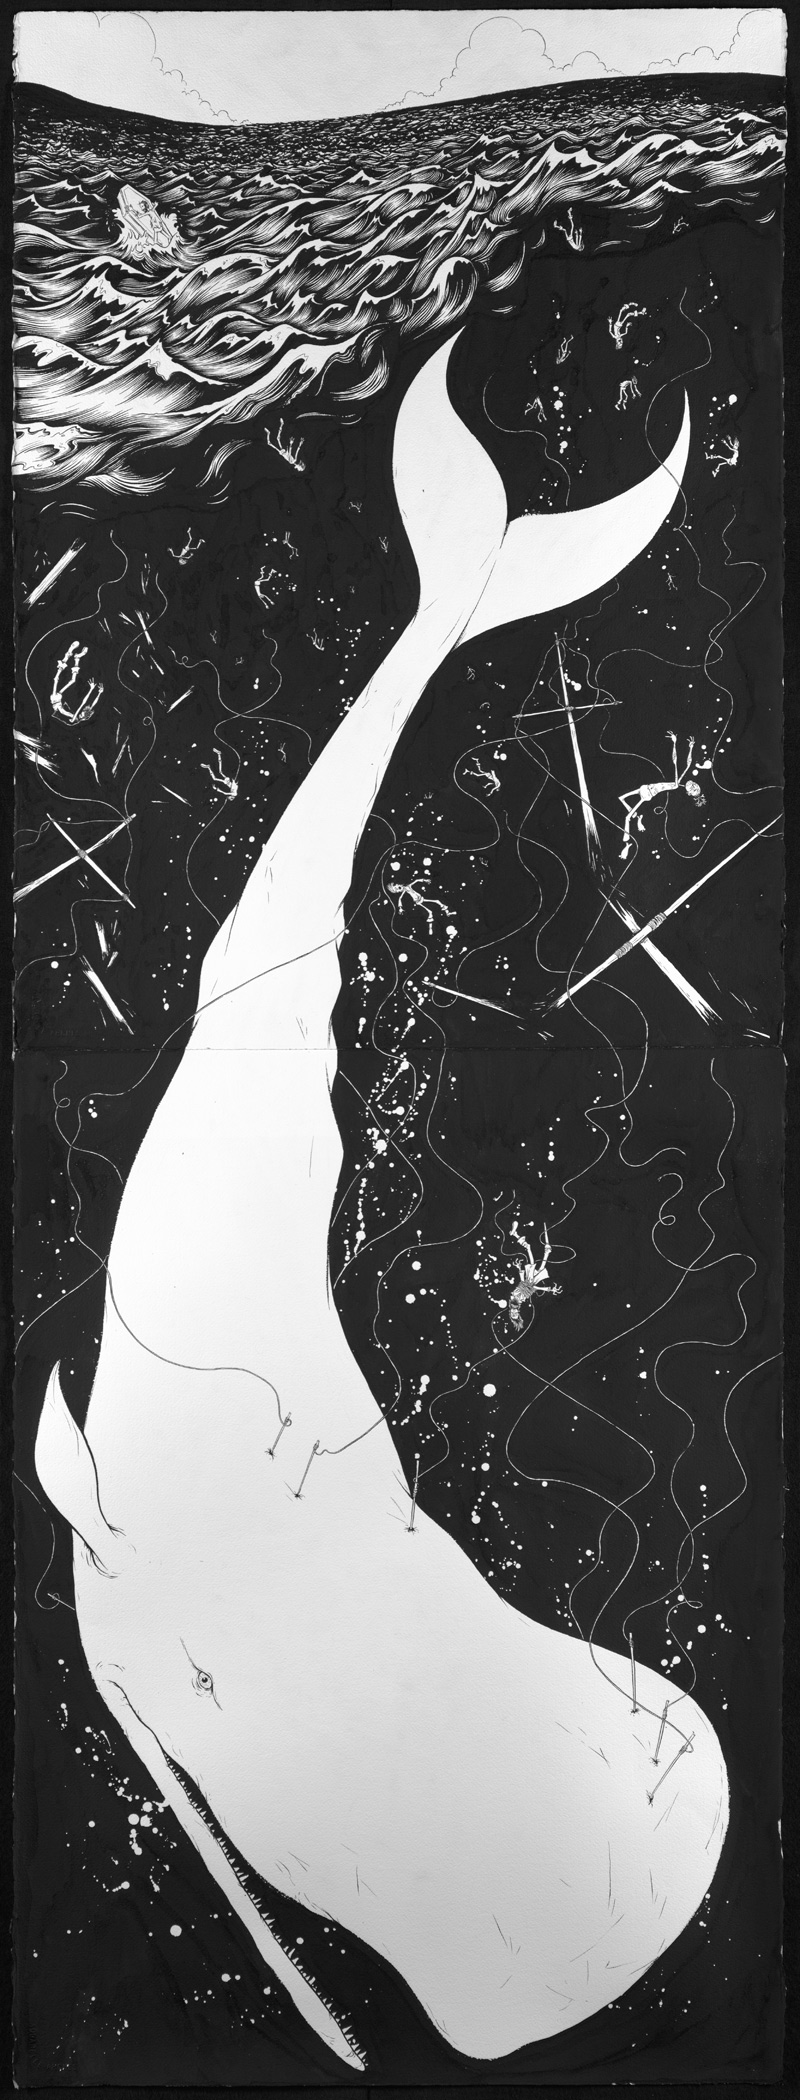
\includegraphics{moby_dick_11}
    \caption{
        \textbf{Moby Dick, or, the Whale.}
My soul is more than matched; she's overmanned; and by a madman! Insufferable sting, that sanity should ground arms on such a field! But he drilled deep down, and blasted all my reason out of me! I think I see his impious end; but feel that I must help him to it. Will I, nill I, the ineffable thing has tied me to him; tows me with a cable I have no knife to cut. Horrible old man! Who's over him, he cries;—aye, he would be a democrat to all above; look, how he lords it over all below! Oh! I plainly see my miserable office,—to obey, rebelling; and worse yet, to hate with touch of pity! For in his eyes I read some lurid woe would shrivel me up, had I it. Yet is there hope. Time and tide flow wide. The hated whale has the round watery world to swim in, as the small gold-fish has its glassy globe. His heaven-insulting purpose, God may wedge aside. I would up heart, were it not like lead. But my whole clock's run down; my heart the all-controlling weight, I have no key to lift again. 
    }
  \end{center}
\end{figure}

   There is, one knows not what sweet mystery about this sea, whose gently awful stirrings seem to speak of some hidden soul beneath; like those fabled undulations of the Ephesian sod over the buried Evangelist St. John. And meet it is, that over these sea- pastures, wide-rolling watery prairies and Potters' Fields of all four continents, the waves should rise and fall, and ebb and flow unceasingly; for here, millions of mixed shades and shadows, drowned dreams, somnambulisms, reveries; all that we call lives and souls, lie dreaming, dreaming, still; tossing like slumberers in their beds; the ever-rolling waves but made so by their restlessness.

   To any meditative Magian rover, this serene Pacific, once beheld, must ever after be the sea of his adoption. It rolls the midmost waters of the world, the Indian ocean and Atlantic being but its arms. The same waves wash the moles of the new-built Californian towns, but yesterday planted by the recentest race of men, and lave the faded but still gorgeous skirts of Asiatic lands, older than Abraham; while all between float milky-ways of coral isles, and low-lying, endless, unknown Archipelagoes, and impenetrable Japans. Thus this mysterious, divine Pacific zones the world's whole bulk about; makes all coasts one bay to it; seems the tide-beating heart of earth. Lifted by those eternal swells, you needs must own the seductive god, bowing your head to Pan.

   But few thoughts of Pan stirred Ahab's brain, as standing like an iron statue at his accustomed place beside the mizen
rigging, with one nostril he unthinkingly snuffed the sugary musk from the Bashee isles (in whose sweet woods mild lovers must be walking), and with the other consciously inhaled the salt breath of the new found sea; that sea in which the hated White Whale must even then be swimming. Launched at length upon these almost final waters, and gliding towards the Japanese cruising-ground, the old man's purpose intensified itself. His firm lips met like the lips of a vice; the Delta of his forehead's veins swelled like overladen brooks; in his very sleep, his ringing cry ran through the vaulted hull, Stern all! the White Whale spouts thick blood! 

\section{Cistern and Buckets}


 Nimble as a cat, Tashtego mounts aloft; and without altering his erect posture, runs straight out upon the overhanging mainyard-arm, to the part where it exactly projects over the hoisted Tun. He has carried with him a light tackle called a whip, consisting of only two parts, travelling through a single-sheaved block. Securing this block, so that it hangs down from the yard-arm, he swings one end of the rope, till it is caught and firmly held by a hand on deck. Then, hand-over-hand, down the other part, the Indian drops through the air, till dexterously he lands on the summit of the head. There—still high elevated above the rest of the company, to whom he vivaciously cries—he seems some Turkish Muezzin calling the good people to prayers from the top of a tower. A short-handled sharp spade being sent up to him, he diligently searches for the proper place to begin breaking into the Tun. In this business he proceeds very heedfully, like a treasure-hunter in some old house, sounding the walls to find where the gold is masoned in. By the time this cautious search is over, a stout iron-bound bucket, precisely like a well-bucket, has been attached to one end of the whip; while the other end, being stretched across the deck, is there held by two or three alert hands. These last now hoist the bucket within grasp of the Indian, to whom another person has reached up a very long pole. Inserting this pole into the bucket, Tashtego downward guides the bucket into the Tun, till it entirely disappears; then giving the word to the seamen at the whip, up comes the bucket again, all bubbling like a dairy-maid's pail of new milk. Carefully lowered from its height, the full-freighted vessel is caught by an appointed hand, and quickly emptied into a large tub. Then remounting aloft, it again goes through the same round until the deep cistern will yield no more. Towards the end, Tashtego has to ram his long pole harder and harder, and deeper and deeper into the Tun, until some twenty feet of the pole have gone down.

Now, the people of the Pequod had been baling some time in this way; several tubs had been filled with the fragrant sperm; when all at once a queer accident happened. Whether it was that Tashtego, that wild Indian, was so heedless and reckless as to let go for a moment his one-handed hold on the great cabled tackles suspending the head; or whether the place where he stood was so treacherous and oozy; or whether the Evil One himself would have it to fall out so, without stating his particular reasons; how it was exactly, there is no telling now; but, on a sudden, as the eightieth or ninetieth bucket came suckingly up—my God! poor Tashtego—like the twin reciprocating bucket in a veritable well, dropped head-foremost down into this great Tun of Heidelburgh, and with a horrible oily gurgling, went clean out of sight!

"Man overboard!" cried Daggoo, who amid the general consternation first came to his senses. "Swing the bucket this way!" and putting one foot into it, so as the better to secure his slippery hand-hold on the whip itself, the hoisters ran him high up to the top of the head, almost before Tashtego could have reached its interior bottom. Meantime, there was a terrible tumult. Looking over the side, they saw the before lifeless head throbbing and heaving just below the surface of the sea, as if that moment seized with some momentous idea; whereas it was only the poor Indian unconsciously revealing by those struggles the perilous depth to which he had sunk.

At this instant, while Daggoo, on the summit of the head, was clearing the whip—which had somehow got foul of the great cutting tackles—a sharp cracking noise was heard; and to the unspeakable horror of all, one of the two enormous hooks suspending the head tore out, and with a vast vibration the enormous mass sideways swung, till the drunk ship reeled and shook as if smitten by an iceberg. The one remaining hook, upon which the entire strain now depended, seemed every instant to be on the point of giving way; an event still more likely from the violent motions of the head.

\begin{figure}[!htp]
  \begin{center}
      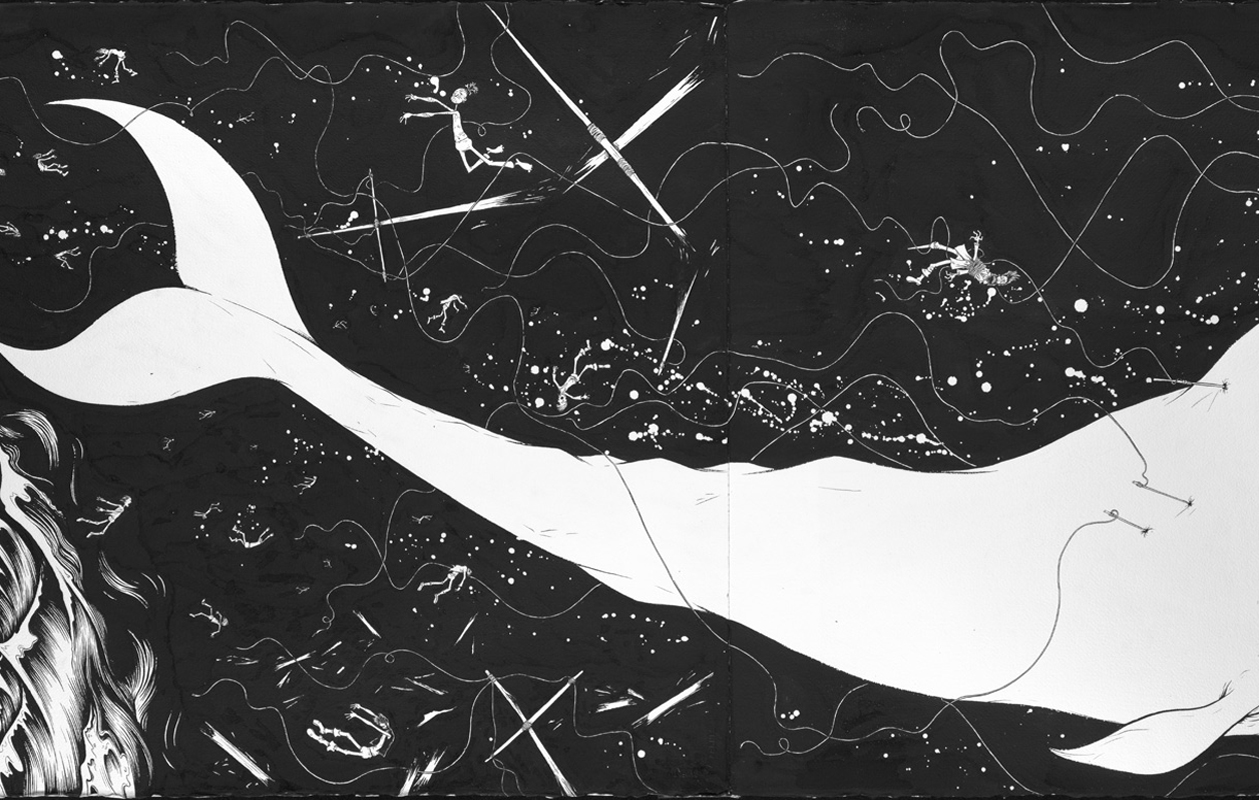
\includegraphics{MOBYDICK}
    \caption{
        \textbf{Moby Dick, or, the Whale.}
My soul is more than matched; she's overmanned; and by a madman! Insufferable sting, that sanity should ground arms on such a field! But he drilled deep down, and blasted all my reason out of me! I think I see his impious end; but feel that I must help him to it. Will I, nill I, the ineffable thing has tied me to him; tows me with a cable I have no knife to cut. Horrible old man! Who's over him, he cries;—aye, he would be a democrat to all above; look, how he lords it over all below! Oh! I plainly see my miserable office,—to obey, rebelling; and worse yet, to hate with touch of pity! For in his eyes I read some lurid woe would shrivel me up, had I it. Yet is there hope. Time and tide flow wide. The hated whale has the round watery world to swim in, as the small gold-fish has its glassy globe. His heaven-insulting purpose, God may wedge aside. I would up heart, were it not like lead. But my whole clock's run down; my heart the all-controlling weight, I have no key to lift again. 
    }
  \end{center}
\end{figure}

"Come down, come down!" yelled the seamen to Daggoo, but with one hand holding on to the heavy tackles, so that if the head should drop, he would still remain suspended; the negro having cleared the foul line, rammed down the bucket into the now collapsed well, meaning that the buried harpooneer should grasp it, and so be hoisted out.

"In heaven's name, man," cried Stubb, "are you ramming home a cartridge there?—Avast! How will that help him; jamming that iron-bound bucket on top of his head? Avast, will ye!"

"Stand clear of the tackle!" cried a voice like the bursting of a rocket.

Almost in the same instant, with a thunder-boom, the enormous mass dropped into the sea, like Niagara's Table-Rock into the whirlpool; the suddenly relieved hull rolled away from it, to far down her glittering copper; and all caught their breath, as half swinging—now over the sailors' heads, and now over the water—Daggoo, through a thick mist of spray, was dimly beheld clinging to the pendulous tackles, while poor, buried-alive Tashtego was sinking utterly down to the bottom of the sea! But hardly had the blinding vapour cleared away, when a naked figure with a boarding-sword in his hand, was for one swift moment seen hovering over the bulwarks. The next, a loud splash announced that my brave Queequeg had dived to the rescue. One packed rush was made to the side, and every eye counted every ripple, as moment followed moment, and no sign of either the sinker or the diver could be seen. Some hands now jumped into a boat alongside, and pushed a little off from the ship.

"Ha! ha!" cried Daggoo, all at once, from his now quiet, swinging perch overhead; and looking further off from the side, we saw an arm thrust upright from the blue waves; a sight strange to see, as an arm thrust forth from the grass over a grave.

"Both! both!—it is both!"—cried Daggoo again with a joyful shout; and soon after, Queequeg was seen boldly striking out with one hand, and with the other clutching the long hair of the Indian. Drawn into the waiting boat, they were quickly brought to the deck; but Tashtego was long in coming to, and Queequeg did not look very brisk.

Now, how had this noble rescue been accomplished? Why, diving after the slowly descending head, Queequeg with his keen sword had made side lunges near its bottom, so as to scuttle a large hole there; then dropping his sword, had thrust his long arm far inwards and upwards, and so hauled out poor Tash by the head. He averred, that upon first thrusting in for him, a leg was presented; but well knowing that that was not as it ought to be, and might occasion great trouble;—he had thrust back the leg, and by a dexterous heave and toss, had wrought a somerset upon the Indian; so that with the next trial, he came forth in the good old way—head foremost. As for the great head itself, that was doing as well as could be expected.

And thus, through the courage and great skill in obstetrics of Queequeg, the deliverance, or rather, delivery of Tashtego, was successfully accomplished, in the teeth, too, of the most untoward and apparently hopeless impediments; which is a lesson by no means to be forgotten. Midwifery should be taught in the same course with fencing and boxing, riding and rowing.

I know that this queer adventure of the Gay-Header's will be sure to seem incredible to some landsmen, though they themselves may have either seen or heard of some one's falling into a cistern ashore; an accident which not seldom happens, and with much less reason too than the Indian's, considering the exceeding slipperiness of the curb of the Sperm Whale's well.

But, peradventure, it may be sagaciously urged, how is this? We thought the tissued, infiltrated head of the Sperm Whale, was the lightest and most corky part about him; and yet thou makest it sink in an element of a far greater specific gravity than itself. We have thee there. Not at all, but I have ye; for at the time poor Tash fell in, the case had been nearly emptied of its lighter contents, leaving little but the dense tendinous wall of the well—a double welded, hammered substance, as I have before said, much heavier than the sea water, and a lump of which sinks in it like lead almost. But the tendency to rapid sinking in this substance was in the present instance materially counteracted by the other parts of the head remaining undetached from it, so that it sank very slowly and deliberately indeed, affording Queequeg a fair chance for performing his agile obstetrics on the run, as you may say. Yes, it was a running delivery, so it was.

Now, had Tashtego perished in that head, it had been a very precious perishing; smothered in the very whitest and daintiest of fragrant spermaceti; coffined, hearsed, and tombed in the secret inner chamber and sanctum sanctorum of the whale. Only one sweeter end can readily be recalled—the delicious death of an Ohio honey-hunter, who seeking honey in the crotch of a hollow tree, found such exceeding store of it, that leaning too far over, it sucked him in, so that he died embalmed. How many, think ye, have likewise fallen into Plato's honey head, and sweetly perished there?




\end{document}
